\documentclass{article}

% don't forget to rotate this document to irritate everyone
% nvm lol, did too good of a job.

\usepackage[top=20mm, bottom=20mm, right=20mm, left=20mm]{geometry}
\usepackage{fancyhdr}
\usepackage{multicol}
\usepackage{amssymb}
\usepackage{tikz}
\usetikzlibrary{intersections}
\usetikzlibrary{calc}
\usepackage{tcolorbox}
\tcbuselibrary{theorems}

\title{The Most \textit{aerodynamic} \textsc{Frisbee} hairstyle.}
\author{Aayush Baj\textbf{aj}}
\date{\today}


\fancyhf{}

\begin{document}

\maketitle
\thispagestyle{fancy}
\dotfill


\providecommand\theoremnumber{}
\newtcbtheorem{Propositionbase}{Proposition \theoremnumber}{colback=purple!5,colframe=gray!100!,fonttitle=\bfseries}{Th}
\newenvironment{Proposition}[1]
 {\renewcommand{\theoremnumber}{#1}\begin{Propositionbase*}}
 {\end{Propositionbase*}}

\begin{Proposition}{1}{}
    The most aerodynamic haircut is that which makes the individual look most like a circle.
    \centering
    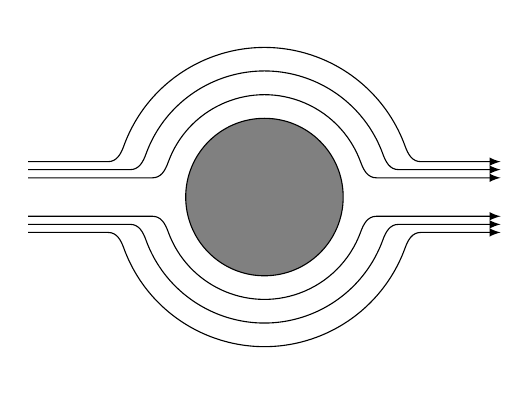
\begin{tikzpicture}[rotate=270]
\filldraw [black,fill=gray] (0,0) circle (1);
\path (0,-3) coordinate (low) (0,3) coordinate (high);
\begin{scope}[overlay]
\foreach \X in {250,290}
{\path[name path global=\X-ray] (0,0) -- (\X:3);}
\end{scope}
\foreach \Z [count=\Y]in {0.3,0.6,0.9}
{\path[name path=circle-\Y] (0,0) circle(1+\Z);
\foreach \X in {250,290}
{\path[name intersections={of=\X-ray and circle-\Y,by=P-\Y-\X}];}
\draw[-latex] ([xshift=2mm]P-\Y-250 |-low) -- 
([xshift=2mm,yshift=-2mm]P-\Y-250) to[out=90,in=-20] (P-\Y-250)
arc(-110:-250:1+\Z) to[out=20,in=-90] ++(0.2,0.2) -- ([xshift=2mm]P-\Y-250 |-high);
\draw[-latex] ([xshift=-2mm]P-\Y-290 |-low) -- 
([xshift=-2mm,yshift=-2mm]P-\Y-290) to[out=90,in=-160] (P-\Y-290)
arc(-70:70:1+\Z) to[out=160,in=-90] ++(-0.2,0.2) -- ([xshift=-2mm]P-\Y-290 |-high);
}
\end{tikzpicture}  

\end{Proposition}

\dotfill\newline

\fbox{
\begin{minipage}{0.9\textwidth}
    \begin{center} \large\textbf{\huge Be like water.} \end{center}
    \begin{flushright}--- Bruce Lee\end{flushright}
\end{minipage}
}

\vspace{1cm}
\begin{minipage}{\textwidth}
    \centering
    \hspace{-1.5cm}
    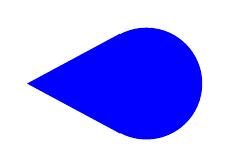
\begin{tikzpicture}[rotate=90]
        \coordinate (a) at (0,1.5);% Change 1.5 to change the shape of the droplet
        \node [circle,draw,fill=blue,blue] (c) at (0,0) [minimum size=40pt] {$c$};
        \draw[blue,fill] (a) -- (tangent cs:node=c,point={(a)},solution=1) --
        (c.center) -- (tangent cs:node=c,point={(a)},solution=2) -- cycle;
    \end{tikzpicture}
\end{minipage}

\vspace{1cm}
\dotfill
\vspace{1cm}

\begin{minipage}{\textwidth}
    \begin{multicols}{2}
    \hspace{4cm}
        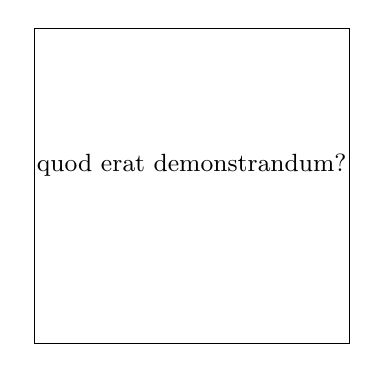
\begin{tikzpicture}
            \draw (0,0) -- (4,0) -- (4,4) -- (0,4) -- (0,0);
              \node at (2,2) [above] {\small quod erat demonstrandum?};
        \end{tikzpicture}
        \begin{tikzpicture}[scale=0.6]

\draw[line width=0.5,line cap=round] (1.5,0) .. controls ++(0,2) and ++(0,-2) .. (4,4)
                                             to[out=90,in=0] (2,6)
                                             to[out=180,in=90] (0,4);

\fill (1.5,-1) circle (0.25);

\end{tikzpicture}
    \end{multicols}
\end{minipage}

\vspace{1cm}
\dotfill

\newpage

\fbox{
\begin{minipage}{0.9\textwidth}
    \begin{center} \large\textbf{\huge Manu et mente} \end{center}
        \begin{flushright}--- Some Nerds (probably)\end{flushright}
\end{minipage}
}

\vspace{0.5cm}

\centering{
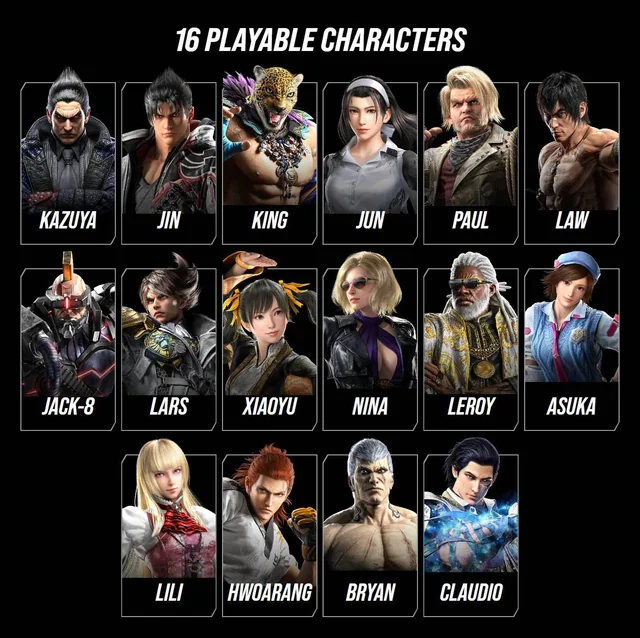
\includegraphics[width=0.8\textwidth]{tekken.png}
\\
}
\vspace{0.5cm}
\

\includegraphics[width=0.5\textwidth]{kazuya.png}
\flushright{
    \begin{math}\therefore \text{ Proposition 1 is False. } \blacksquare\end{math}
}




\end{document}


